% ------------------------------------------------------------------------------
% TYPO3 CMS 6.2 LTS - What's New - Chapter "TypoScript" (Spanish Version)
%
% @author	Sergio Catalá <sergio.catala@e-net.info>
% @author	Michel Mix <mmix@autistici.org>
% @license	Creative Commons BY-NC-SA 3.0
% @link		http://typo3.org/download/release-notes/whats-new/
% @language	Spanish
% ------------------------------------------------------------------------------
% Chapter: TypoScript
% ------------------------------------------------------------------------------

\section{TSconfig y TypoScript}
\begin{frame}[fragile]
	\frametitle{TSconfig y TypoScript}

	\begin{center}\huge{Capítulo 4:}\end{center}
	\begin{center}\huge{\color{typo3darkgrey}\textbf{TSconfig y TypoScript}}\end{center}

\end{frame}

% ------------------------------------------------------------------------------
% Include TypoScript
% ------------------------------------------------------------------------------
% http://forge.typo3.org/issues/34621

\begin{frame}[fragile]
	\frametitle{TSconfig y TypoScript}
	\framesubtitle{Incluir TypoScript (1)}

	\begin{itemize}
		\item Incluya todos los ficheros TypoScript desde un directorio (recursivo)

			\lstinline!<INCLUDE_TYPOSCRIPT: source="DIR:directory">!
			\lstinline!<INCLUDE_TYPOSCRIPT: source="DIR:EXT:myextension/res/setup">!

		\item Orden en el que los ficheros son incluidos:\newline
			alfabéticamente, primero ficheros, luego directorios
		\item Limite ficheros a incluir añadiendo \texttt{extensions="..."}

			\lstinline!<INCLUDE_TYPOSCRIPT: source="DIR:directory" extensions="ts">!

		\item Por defecto, sólo pueden incluirse ficheros con extensiones ts, t3, t3s, t3c, txt
		\item Esta lista es configurable (Herramienta de Instalación):\newline
			\texttt{\$TYPO3\_CONF\_VARS['SYS']['tsfile\_ext']}
	\end{itemize}

\end{frame}

% ------------------------------------------------------------------------------
% Include TypoScript
% ------------------------------------------------------------------------------
% http://forge.typo3.org/issues/52018

\begin{frame}[fragile]
	\frametitle{TSconfig y TypoScript}
	\framesubtitle{Incluir TypoScript (2)}

	\begin{itemize}
		\item Pueden pasarse rutas relativas a \texttt{INCLUDE\_TYPOSCRIPT},\newline
			si se llama a la inclusión recursivamente desde un fichero
		\item La primera inclusión \textbf{debe ser} absoluta
		\item \texttt{./} refleja el directorio actual de la última inclusión
		\item \texttt{../} refleja el directorio padre de la última inclusión
		\item Ejemplos:

			\lstinline!<INCLUDE_TYPOSCRIPT: source="FILE:directory/typoscript/setup.ts">!
			\lstinline!<INCLUDE_TYPOSCRIPT: source="FILE:./filename.ts">!
			\lstinline!<INCLUDE_TYPOSCRIPT: source="FILE:../filename.ts">!
			\lstinline!<INCLUDE_TYPOSCRIPT: source="FILE:../directory/filename.ts">!

	\end{itemize}

\end{frame}

% ------------------------------------------------------------------------------
% stdWrap for strPad
% ------------------------------------------------------------------------------
% http://forge.typo3.org/issues/43604

\begin{frame}[fragile]
	\frametitle{TSconfig y TypoScript}
	\framesubtitle{strPad}

	\begin{itemize}
		\item Se ha añadido \texttt{stdWrap} a las propiedades de \texttt{strPad}

			\begin{lstlisting}
				page = PAGE
				page.10 = TEXT
				page.10 {
				  value = Hello World!
				  strPad {
				    length = 5
				    length {
				      current = 1
				      setCurrent.data = TSFE:page|uid
				      setCurrent.wrap = | + 80
				      prioriCalc = 1
				    }
				    padWith = .
				  }
				}
			\end{lstlisting}

	\end{itemize}

\end{frame}

% ------------------------------------------------------------------------------
% stdWrap for _DEFAULT_PI_VARS
% ------------------------------------------------------------------------------
% http://forge.typo3.org/issues/22045
% http://forge.typo3.org/issues/49314

\begin{frame}[fragile]
	\frametitle{TSconfig y TypoScript}
	\framesubtitle{\_DEFAULT\_PI\_VARS}

	\begin{itemize}
		\item Se ha añadido \texttt{stdWrap} para \texttt{\_DEFAULT\_PI\_VARS}
		\item \texttt{\_DEFAULT\_PI\_VARS} son usadas para fijar valores por defecto para piVars (variables GET/POST para una extensión)

		\item TYPO3 < 6.2
			\begin{lstlisting}
				plugin.tt_news._DEFAULT_PI_VARS {
				  year = 2013
				}
			\end{lstlisting}

		\item TYPO3 >= 6.2
			\begin{lstlisting}
				plugin.tt_news._DEFAULT_PI_VARS {
				  year.stdWrap.data = date:Y
				}
			\end{lstlisting}

	\end{itemize}

\end{frame}

% ------------------------------------------------------------------------------
% Debug Register and Page
% ------------------------------------------------------------------------------
% http://forge.typo3.org/issues/49478

\begin{frame}[fragile]
	\frametitle{TSconfig y TypoScript}
	\framesubtitle{Salida de Depuración}

	\begin{columns}[T]

		\begin{column}{.6\textwidth}
			\begin{itemize}
				\item Salida de depuración para el registro y variables de páginas:\newline
					\texttt{\$GLOBALS['TSFE']->register}\newline
					\texttt{\$GLOBALS['TSFE']->page}

				\item Ejemplos:

					\begin{lstlisting}
						10 = LOAD_REGISTER
						10.variable = value
					\end{lstlisting}

					\begin{lstlisting}
						20 = TEXT
						20.data = debug:register
					\end{lstlisting}

					\begin{lstlisting}
						30 = TEXT
						30.data = debug:page
					\end{lstlisting}

			\end{itemize}
		\end{column}

		\begin{column}{.4\textwidth}
			\begin{figure}\vspace*{-0.4cm}
				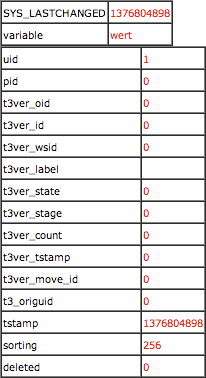
\includegraphics[width=0.6\linewidth]{Images/TypoScript/DebugRegisterAndPage.png}
			\end{figure}
		\end{column}

	\end{columns}

\end{frame}

% ------------------------------------------------------------------------------
% File Links: "register:titleText" and "register:altText"
% ------------------------------------------------------------------------------
% http://forge.typo3.org/issues/44182

\begin{frame}[fragile]
	\frametitle{TSconfig y TypoScript}
	\framesubtitle{Enlaces de Ficheros}

	\begin{itemize}
		\item Los enlaces de fichero ofrecen una descripción, un texto de título y un texto de etiqueta alternativa para cada fichero.
			Pueden accederse a los tres vía registros:

			\begin{itemize}
				\item \texttt{register:description}
				\item \texttt{register:titleText}
				\item \texttt{register:altText}
			\end{itemize}

		\item Ejemplo:

			\begin{lstlisting}
				# filelinks
				tt_content.uploads.20 {
				  # link description instead of filename
				  labelStdWrap.data = register:description
				  # output alternative text
				  itemRendering.20.data = register:titleText
				}
			\end{lstlisting}

	\end{itemize}

\end{frame}

% ------------------------------------------------------------------------------
% stdWrap replacement: add optionSplit-support
% ------------------------------------------------------------------------------
% http://forge.typo3.org/issues/42287

\begin{frame}[fragile]
	\frametitle{TSconfig y TypoScript}
	\framesubtitle{Función stdWrap: reemplazo (1)}

	\begin{itemize}
		\item Opción \texttt{replace} de la función \texttt{stdWrap} \texttt{replacement}\newline
			soporta ahora \texttt{optionSplit}

		\item Ejemplo 1:

			\begin{lstlisting}
				10 = TEXT
				10.value = TYPO3_inspires_people_to_share
				10.replacement.10 {
				  search = _
				  replace = 1 || 2 || 3
				  useOptionSplitReplace = 1
				}
			\end{lstlisting}

			Salida:\newline
				\texttt{TYPO31inspires2people3to3share}

	\end{itemize}

\end{frame}

% ------------------------------------------------------------------------------
% stdWrap replacement: add optionSplit-support
% ------------------------------------------------------------------------------
% http://forge.typo3.org/issues/42287

\begin{frame}[fragile]
	\frametitle{TSconfig y TypoScript}
	\framesubtitle{Función stdWrap: reemplazo (2)}

	\begin{itemize}
		\item Opción \texttt{replace} de la función \texttt{stdWrap} \texttt{replacement}\newline
			soporta ahora \texttt{optionSplit}

		\item Ejemplo 2:

			\begin{lstlisting}
				10 = TEXT
				10.value = TYPO3 inspires people to share
				10.replacement.10 {
				  search = #(TYPO3|people|share)#i
				  replace = ${1} CMS || all ${1} || collaborate and ${1}
				  useOptionSplitReplace = 1
				  useRegExp = 1
				}
			\end{lstlisting}

			Salida:\newline
				\texttt{TYPO3 CMS inspires all people to collaborate and share}

	\end{itemize}

\end{frame}

% ------------------------------------------------------------------------------
% Register values in FilesContentObject
% ------------------------------------------------------------------------------
% http://forge.typo3.org/issues/49480

\begin{frame}[fragile]
	\frametitle{TSconfig y TypoScript}
	\framesubtitle{cObject FILE}

	\begin{itemize}
		\item Dos registros añadidos a cObject FILES:\newline
			\texttt{FILE\_NUM\_CURRENT} y \texttt{FILES\_COUNT}

		\item Ejemplo:

			\lstset{
				basicstyle=\tiny\ttfamily
			}

			\begin{lstlisting}
				10 = FILES
				10 {
				  references {
				    table = tt_news
				    uid.field = uid
				    fieldName = media
				  }
				  renderObj = COA
				  renderObj {
				    10 = TEXT
				    10.value = Renders first file twice
				    10.if.isFalse.data = register:FILE_NUM_CURRENT
				    20 = TEXT
				    20.value = file {register:FILE_NUM_CURRENT} of {register:FILES_COUNT}
				    20.insertData = 1
				  }
				}
			\end{lstlisting}

	\end{itemize}

\end{frame}

% ------------------------------------------------------------------------------
% Category Menu In TypoScript
% ------------------------------------------------------------------------------
% http://forge.typo3.org/issues/51161

\begin{frame}[fragile]
	\frametitle{TSconfig y TypoScript}
	\framesubtitle{Menú de Categoría}

	\begin{itemize}
		\item se puede generar un menú de categorías en TypoScript

		\item Ejemplo:

			\lstset{
				basicstyle=\tiny\ttfamily
			}

			\begin{lstlisting}
				page.20 = HMENU
				page.20 {
				  special = categories
				  special {
				    # comma-separated list of categories
				    value = 1
				    # sort by title (stdWrap)
				    sorting = title
				    # sorting "asc" or "desc" (stdWrap)
				    order = desc
				    1 = TMENU
				    1.NO {
				      allWrap = <li> | </li>
				    }
				  }
				}
			\end{lstlisting}

	\end{itemize}

\end{frame}

% ------------------------------------------------------------------------------
% cObject RECORDS with category support
% (slide added in March 2014)
% ------------------------------------------------------------------------------

\begin{frame}[fragile]
	\frametitle{TSconfig y TypoScript}
	\framesubtitle{Categorías de Acceso}

	\begin{itemize}
		\item Propiedad \texttt{categories} permite el acceso a categorías\newline
			para los cObject RECORDS

		\item Ejemplo:

			\lstset{
				basicstyle=\tiny\ttfamily
			}

			\begin{lstlisting}
				# menu of categorized content elements
				categorized_content = RECORDS
				categorized_content {
				  categories.field = selected_categories
				  categories.relation.field = category_field
				  tables = tt_content
				  conf.tt_content = TEXT
				  conf.tt_content {
				    field = header
				    typolink.parameter = {field:pid}#{field:uid}
				    typolink.parameter.insertData = 1
				    wrap = <li>|</li>
				  }
				  wrap = <ul>|</ul>
				}
			\end{lstlisting}

	\end{itemize}

\end{frame}

% ------------------------------------------------------------------------------
% Category Menu In TypoScript
% ------------------------------------------------------------------------------
% http://forge.typo3.org/issues/51782

\begin{frame}[fragile]
	\frametitle{TSconfig y TypoScript}
	\framesubtitle{Ficheros CSS y JavaScript}

	\begin{itemize}
		\item \texttt{splitChar} puede definirse ahora para las propiedades \texttt{allWrap}
		\item Wrap funciona ahora como el método estándar \texttt{stdWrap.wrap}
		\item Carácter \texttt{splitChar} por defecto es el símbolo de tubería: \texttt{|}
		\item Este cambio afecta:

			\begin{itemize}
				\item \texttt{includeCSS}
				\item \texttt{includeJSlibs}
				\item \texttt{includeJSFooterlibs}
				\item \texttt{includeJS}
				\item \texttt{includeJSFooter}
			\end{itemize}

	\end{itemize}

\end{frame}


% ------------------------------------------------------------------------------
% Conditions: userFunc Accepts Multiple Arguments
% ------------------------------------------------------------------------------
% http://forge.typo3.org/issues/47159

\begin{frame}[fragile]
	\frametitle{TSconfig y TypoScript}
	\framesubtitle{Condiciones (1)}

	\begin{itemize}
		\item Condición \texttt{userFunc} acepta ahora múltiples argumentos

		\item TYPO3 < 6.2
			\begin{lstlisting}
				[userFunc = user_function(argument1)]
			\end{lstlisting}

		\item TYPO3 >= 6.2
			\begin{lstlisting}
				[userFunc = user_function(argument1, argument2, ...)]
			\end{lstlisting}

		\item Ejemplo:
			% \texttt{[userFunc = user\_match(checkSubnet, 192.168)]}

			\lstinline![userFunc = user_match(checkSubnet, 192.168)]!

			\begin{lstlisting}
				function user_match($command, $subnet) {
				  switch($command) {
				    case 'checkSubnet':
				      if (strstr(getenv('REMOTE_ADDR'), $subnet)) { ... }
				  }
				}
			\end{lstlisting}

	\end{itemize}

\end{frame}

% ------------------------------------------------------------------------------
% Conditions: Application Context
% ------------------------------------------------------------------------------
% http://forge.typo3.org/issues/39441
% http://forge.typo3.org/issues/50132

\begin{frame}[fragile]
	\frametitle{TSconfig y TypoScript}
	\framesubtitle{Condiciones (2)}

	\begin{itemize}
		\item Puede determinarse el contexto de la aplicación en condiciones
		\item Se soportan comodines "\texttt{+}" y "\texttt{*}" y expresiones regulares
		\item Ejemplos:

			\lstset{
				basicstyle=\tiny\ttfamily
			}

			\begin{lstlisting}
				[applicationContext = Development/Debugging, Development/Profiling]
				  # Sitio TYPO3 en fase Development
				[global]

				[applicationContext = Production*]
				  # Sitio TYPO3 en fase Production
				  # por ejemplo "Production/Live" o "Production/Staging"
				[global]

				[applicationContext = /^TestServer\d+$/]
				  # Sitio TYPO3 en TestServer1 o TestServer2 o TestServer3, etc.
				[global]
			\end{lstlisting}

	\end{itemize}

\end{frame}

% ------------------------------------------------------------------------------
% Conditions: IP Supports Keyword devIP
% ------------------------------------------------------------------------------
% http://forge.typo3.org/issues/50092

\begin{frame}[fragile]
	\frametitle{TSconfig y TypoScript}
	\framesubtitle{Condiciones (3)}

	\begin{itemize}

		\item Al usar una condición IP, puede usarse la palabra clave \texttt{devIP} para chequear si la dirección IP del cliente concuerda con el ajuste \texttt{devIpMask} de la Herramienta de Instalación
		\item Ejemplo:

%			\lstset{
%				basicstyle=\tiny\ttfamily
%			}

			\begin{lstlisting}
				[IP = devIP]
				  page.10 = TEXT
				  page.10.value = Hello Developer!
				[global]
			\end{lstlisting}

	\end{itemize}

\end{frame}

% ------------------------------------------------------------------------------
% Records Without Default Translation
% ------------------------------------------------------------------------------
% http://forge.typo3.org/issues/24005

\begin{frame}[fragile]
	\frametitle{TSconfig y TypoScript}
	\framesubtitle{Registros Sin Traducción por Defecto}

	\begin{itemize}

		\item Nueva opción \texttt{includeRecordsWithoutDefaultTranslation}
			recupera registros sin un padre de localización\newline
			(pero con \texttt{languageField} en base al lenguaje actual)

		\item Ejemplo:

			\begin{lstlisting}
				pageContent = CONTENT
				pageContent {
				  table = tt_content
				  select.includeRecordsWithoutDefaultTranslation = 1
				  ...
				}
			\end{lstlisting}

	\end{itemize}

\end{frame}

% ------------------------------------------------------------------------------
% cObject FILES: begin/maxItems options
% ------------------------------------------------------------------------------
% http://forge.typo3.org/issues/52632

\begin{frame}[fragile]
	\frametitle{TSconfig y TypoScript}
	\framesubtitle{cObject FILES}

	\begin{itemize}

		\item cObject FILES soporta \texttt{begin} y \texttt{maxItems} como propiedades ahora

		\item Ejemplo:

			\lstset{
				basicstyle=\tiny\ttfamily
			}

			\begin{lstlisting}
				page.10 = FILES
				page.10 {
				  references {
				    table = pages
				    uid.data = page:uid
				    fieldName = media
				  }

				  # recupera hasta 5 ficheros, empezando por el primero (0):
				  begin = 0
				  maxItems = 5

				  renderObj = TEXT
				  renderObj {
				    data = file:current:size
				    wrap = <p>File size:<strong>|</strong></p>
				  }
				}
			\end{lstlisting}

	\end{itemize}

\end{frame}

% ------------------------------------------------------------------------------
% Exclude doktypes From Pagetree
% ------------------------------------------------------------------------------
% http://forge.typo3.org/issues/49279
% http://forge.typo3.org/issues/49356

\begin{frame}[fragile]
	\frametitle{TSconfig y TypoScript}
	\framesubtitle{Excluir doktypes Del Árbol de Páginas}

	\begin{itemize}

		\item Pueden excluirse doktypes específicos del árbol de páginas
		\item La configuración sucede en UserTSconfig (por lo tanto, específica del usuario o grupo)
		\item Ejemplos:

			\begin{lstlisting}
				# excluir tipos "carpetas"
				options.pageTree.excludeDoktypes = 254

				# excluir tipos "carpetas" y "standard"
				options.pageTree.excludeDoktypes = 254,1
			\end{lstlisting}

	\end{itemize}

\end{frame}

% ------------------------------------------------------------------------------
% Hide Modules In Backend
% ------------------------------------------------------------------------------

\begin{frame}[fragile]
	\frametitle{TSconfig y TypoScript}
	\framesubtitle{Esconder Módulos en Backend}

	\begin{itemize}

		\item Pueden esconderse módulos en el backend
		\item Esto no repercute en el acceso\newline
			(use el ACL para usuarios y grupos BE para acceso restringido)
		\item Ejemplos:

			\lstinline!options.hideModules = file, help!
			\lstinline!options.hideModules.web := addToList(func,info)!
			\lstinline!options.hideModules.system = BelogLog!

	\end{itemize}

\end{frame}

% ------------------------------------------------------------------------------
% Alternative Domain For Preview
% ------------------------------------------------------------------------------
% http://forge.typo3.org/issues/30889

\begin{frame}[fragile]
	\frametitle{TSconfig y TypoScript}
	\framesubtitle{Dominio de Vista Preliminar}

	\begin{itemize}

		\item Puede fijarse un dominio alternativo para vistas preliminares de página/sitio en PageTS
		\item Útil para sitios multidominio
		\item Ejemplo:

			\lstinline!TCEMAIN.viewDomain = example.com!

	\end{itemize}

\end{frame}

% ------------------------------------------------------------------------------
% Conditions in Backend Layouts
% ------------------------------------------------------------------------------
% http://forge.typo3.org/issues/47588

\begin{frame}[fragile]
	\frametitle{TSconfig y TypoScript}
	\framesubtitle{Condiciones en Diseños del Backend}

	\begin{itemize}

		\item Los diseños del backend ahora soportan condiciones
		\item Ejemplo:

			\lstset{
				basicstyle=\tiny\ttfamily
			}

			\begin{lstlisting}
				backend_layout {
				  colCount = 2
				  rowCount = 1
				  rows {
				    1 {
				      columns {
				        1.name = Main
				        1.colPos = 0
				        2.name = Right
				        2.colPos = 1
				      }
				    }
				  }
				}

				[PIDupinRootline = 123]
				  # remove right column in branch of page ID 123
				  backend_layout.rows.1.columns.2 >
				[global]
			\end{lstlisting}

	\end{itemize}

\end{frame}

% ------------------------------------------------------------------------------
% Miscellaneous
% ------------------------------------------------------------------------------
% http://forge.typo3.org/issues/34597 (showForgotPassword)
% http://forge.typo3.org/issues/50138 (showForgotPassword)
%
% http://forge.typo3.org/issues/19732 (Content-Length)
%
% http://forge.typo3.org/issues/16386 (Indexed Search) - wow: submitted 7 years ago :-)

\begin{frame}[fragile]
	\frametitle{TSconfig y TypoScript}
	\framesubtitle{Varios}

	\begin{itemize}

		\item Desactivar/activar enlace de "contraseña olvidada" a través de la opción \small\texttt{showForgotPassword}\normalsize\newline
			(útil, si se incluyen múltiples formularios de autenticación a través de EXT:felogin en una página)

		\item Respuesta HTTP incluye cabecera \texttt{Content-length} por defecto ahora

			\begin{itemize}
				\item Acelera el renderizado si se activa pipelining en Apache
				\item Puede configurarse a través de \texttt{config.enableContentLengthHeader}
			\end{itemize}

		\item Lista de resultado de EXT:indexed\_search tiene propiedades \texttt{stdWrap}\newline
			(opción: \texttt{plugin.tx\_indexedsearch.resultlist\_stdWrap})

	\end{itemize}

\end{frame}

% ------------------------------------------------------------------------------

